\documentclass[twoside]{book}

% Packages required by doxygen
\usepackage{fixltx2e}
\usepackage{calc}
\usepackage{doxygen}
\usepackage[export]{adjustbox} % also loads graphicx
\usepackage{graphicx}
\usepackage[utf8]{inputenc}
\usepackage{makeidx}
\usepackage{multicol}
\usepackage{multirow}
\PassOptionsToPackage{warn}{textcomp}
\usepackage{textcomp}
\usepackage[nointegrals]{wasysym}
\usepackage[table]{xcolor}

% NLS support packages
\usepackage[french]{babel}

% Font selection
\usepackage[T1]{fontenc}
\usepackage[scaled=.90]{helvet}
\usepackage{courier}
\usepackage{amssymb}
\usepackage{sectsty}
\renewcommand{\familydefault}{\sfdefault}
\allsectionsfont{%
  \fontseries{bc}\selectfont%
  \color{darkgray}%
}
\renewcommand{\DoxyLabelFont}{%
  \fontseries{bc}\selectfont%
  \color{darkgray}%
}
\newcommand{\+}{\discretionary{\mbox{\scriptsize$\hookleftarrow$}}{}{}}

% Page & text layout
\usepackage{geometry}
\geometry{%
  a4paper,%
  top=2.5cm,%
  bottom=2.5cm,%
  left=2.5cm,%
  right=2.5cm%
}
\tolerance=750
\hfuzz=15pt
\hbadness=750
\setlength{\emergencystretch}{15pt}
\setlength{\parindent}{0cm}
\setlength{\parskip}{3ex plus 2ex minus 2ex}
\makeatletter
\renewcommand{\paragraph}{%
  \@startsection{paragraph}{4}{0ex}{-1.0ex}{1.0ex}{%
    \normalfont\normalsize\bfseries\SS@parafont%
  }%
}
\renewcommand{\subparagraph}{%
  \@startsection{subparagraph}{5}{0ex}{-1.0ex}{1.0ex}{%
    \normalfont\normalsize\bfseries\SS@subparafont%
  }%
}
\makeatother

% Headers & footers
\usepackage{fancyhdr}
\pagestyle{fancyplain}
\fancyhead[LE]{\fancyplain{}{\bfseries\thepage}}
\fancyhead[CE]{\fancyplain{}{}}
\fancyhead[RE]{\fancyplain{}{\bfseries\leftmark}}
\fancyhead[LO]{\fancyplain{}{\bfseries\rightmark}}
\fancyhead[CO]{\fancyplain{}{}}
\fancyhead[RO]{\fancyplain{}{\bfseries\thepage}}
\fancyfoot[LE]{\fancyplain{}{}}
\fancyfoot[CE]{\fancyplain{}{}}
\fancyfoot[RE]{\fancyplain{}{\bfseries\scriptsize Généré par Doxygen }}
\fancyfoot[LO]{\fancyplain{}{\bfseries\scriptsize Généré par Doxygen }}
\fancyfoot[CO]{\fancyplain{}{}}
\fancyfoot[RO]{\fancyplain{}{}}
\renewcommand{\footrulewidth}{0.4pt}
\renewcommand{\chaptermark}[1]{%
  \markboth{#1}{}%
}
\renewcommand{\sectionmark}[1]{%
  \markright{\thesection\ #1}%
}

% Indices & bibliography
\usepackage{natbib}
\usepackage[titles]{tocloft}
\setcounter{tocdepth}{3}
\setcounter{secnumdepth}{5}
\makeindex

% Hyperlinks (required, but should be loaded last)
\usepackage{ifpdf}
\ifpdf
  \usepackage[pdftex,pagebackref=true]{hyperref}
\else
  \usepackage[ps2pdf,pagebackref=true]{hyperref}
\fi
\hypersetup{%
  colorlinks=true,%
  linkcolor=blue,%
  citecolor=blue,%
  unicode%
}

% Custom commands
\newcommand{\clearemptydoublepage}{%
  \newpage{\pagestyle{empty}\cleardoublepage}%
}

\usepackage{caption}
\captionsetup{labelsep=space,justification=centering,font={bf},singlelinecheck=off,skip=4pt,position=top}

%===== C O N T E N T S =====

\begin{document}

% Titlepage & ToC
\hypersetup{pageanchor=false,
             bookmarksnumbered=true,
             pdfencoding=unicode
            }
\pagenumbering{alph}
\begin{titlepage}
\vspace*{7cm}
\begin{center}%
{\Large The Super Sayem }\\
\vspace*{1cm}
{\large Généré par Doxygen 1.8.13}\\
\end{center}
\end{titlepage}
\clearemptydoublepage
\pagenumbering{roman}
\tableofcontents
\clearemptydoublepage
\pagenumbering{arabic}
\hypersetup{pageanchor=true}

%--- Begin generated contents ---
\chapter{Index des classes}
\section{Liste des classes}
Liste des classes, structures, unions et interfaces avec une brève description \+:\begin{DoxyCompactList}
\item\contentsline{section}{\hyperlink{structbutton}{button} }{\pageref{structbutton}}{}
\item\contentsline{section}{\hyperlink{structbutton__menu}{button\+\_\+menu} }{\pageref{structbutton__menu}}{}
\item\contentsline{section}{\hyperlink{structea}{ea} }{\pageref{structea}}{}
\item\contentsline{section}{\hyperlink{structenigme}{enigme} }{\pageref{structenigme}}{}
\item\contentsline{section}{\hyperlink{structenigmes}{enigmes} }{\pageref{structenigmes}}{}
\item\contentsline{section}{\hyperlink{structkeymapping}{keymapping} }{\pageref{structkeymapping}}{}
\item\contentsline{section}{\hyperlink{structperso}{perso} }{\pageref{structperso}}{}
\item\contentsline{section}{\hyperlink{structsaving}{saving} }{\pageref{structsaving}}{}
\item\contentsline{section}{\hyperlink{structsettings}{settings} }{\pageref{structsettings}}{}
\item\contentsline{section}{\hyperlink{structstats}{stats} }{\pageref{structstats}}{}
\item\contentsline{section}{\hyperlink{structtest}{test} }{\pageref{structtest}}{}
\end{DoxyCompactList}

\chapter{Documentation des classes}
\hypertarget{structbutton}{}\section{Référence de la structure button}
\label{structbutton}\index{button@{button}}
\subsection*{Attributs publics}
\begin{DoxyCompactItemize}
\item 
\mbox{\Hypertarget{structbutton_a245136de5539a7c34e7709c893b0ce7f}\label{structbutton_a245136de5539a7c34e7709c893b0ce7f}} 
S\+D\+L\+\_\+\+Surface $\ast$ {\bfseries image} \mbox{[}3\mbox{]}
\item 
\mbox{\Hypertarget{structbutton_a283ac65aff45ef683eeabb8c3b65a51a}\label{structbutton_a283ac65aff45ef683eeabb8c3b65a51a}} 
S\+D\+L\+\_\+\+Rect {\bfseries pos}
\end{DoxyCompactItemize}


La documentation de cette structure a été générée à partir du fichier suivant \+:\begin{DoxyCompactItemize}
\item 
menu.\+h\end{DoxyCompactItemize}

\hypertarget{structbutton__menu}{}\section{Référence de la structure button\+\_\+menu}
\label{structbutton__menu}\index{button\+\_\+menu@{button\+\_\+menu}}
\subsection*{Attributs publics}
\begin{DoxyCompactItemize}
\item 
\mbox{\Hypertarget{structbutton__menu_a7ad66410dade1ecaa4e65c0326c0d624}\label{structbutton__menu_a7ad66410dade1ecaa4e65c0326c0d624}} 
S\+D\+L\+\_\+\+Surface $\ast$ {\bfseries image}
\item 
\mbox{\Hypertarget{structbutton__menu_a36367b8751a348ab63653cfc2c9e7ab0}\label{structbutton__menu_a36367b8751a348ab63653cfc2c9e7ab0}} 
S\+D\+L\+\_\+\+Rect {\bfseries pos}
\item 
\mbox{\Hypertarget{structbutton__menu_ac678b43de43c3ec8677c301e9c98061d}\label{structbutton__menu_ac678b43de43c3ec8677c301e9c98061d}} 
int {\bfseries state}
\end{DoxyCompactItemize}


La documentation de cette structure a été générée à partir du fichier suivant \+:\begin{DoxyCompactItemize}
\item 
menu.\+h\end{DoxyCompactItemize}

\hypertarget{structea}{}\section{Référence de la structure ea}
\label{structea}\index{ea@{ea}}
\subsection*{Attributs publics}
\begin{DoxyCompactItemize}
\item 
\mbox{\Hypertarget{structea_a7ad1c0910e9838a81ae71878ca10a11b}\label{structea_a7ad1c0910e9838a81ae71878ca10a11b}} 
S\+D\+L\+\_\+\+Surface $\ast$ {\bfseries image} \mbox{[}2\mbox{]}\mbox{[}5\mbox{]}
\item 
\mbox{\Hypertarget{structea_a49262ff57ab0f98ad2de7217a5eeaa48}\label{structea_a49262ff57ab0f98ad2de7217a5eeaa48}} 
S\+D\+L\+\_\+\+Rect {\bfseries pos}
\item 
\mbox{\Hypertarget{structea_ab90dafb742e4bca460cc08ed35da1246}\label{structea_ab90dafb742e4bca460cc08ed35da1246}} 
int {\bfseries d}
\item 
\mbox{\Hypertarget{structea_a036d0299c9cb669f7d7de4608dc94c58}\label{structea_a036d0299c9cb669f7d7de4608dc94c58}} 
int {\bfseries d1}
\item 
\mbox{\Hypertarget{structea_a47fd200529d0bb95bb09bfafe7f040a6}\label{structea_a47fd200529d0bb95bb09bfafe7f040a6}} 
int {\bfseries num}
\item 
\mbox{\Hypertarget{structea_a3287146d5da3a8aacbe7d7e80825c4ff}\label{structea_a3287146d5da3a8aacbe7d7e80825c4ff}} 
int {\bfseries num\+\_\+animation}
\item 
\mbox{\Hypertarget{structea_afa5ce90b88e2c4f45be16dc54f58203d}\label{structea_afa5ce90b88e2c4f45be16dc54f58203d}} 
int {\bfseries animation\+\_\+speed}
\item 
\mbox{\Hypertarget{structea_afc3791816f43b84937b2df300b75db8e}\label{structea_afc3791816f43b84937b2df300b75db8e}} 
int {\bfseries speed}
\end{DoxyCompactItemize}


La documentation de cette structure a été générée à partir du fichier suivant \+:\begin{DoxyCompactItemize}
\item 
personnage.\+h\end{DoxyCompactItemize}

\hypertarget{structenigme}{}\section{Référence de la structure enigme}
\label{structenigme}\index{enigme@{enigme}}
\subsection*{Attributs publics}
\begin{DoxyCompactItemize}
\item 
\mbox{\Hypertarget{structenigme_afef580eaca259227dac7bbae2d09f8f7}\label{structenigme_afef580eaca259227dac7bbae2d09f8f7}} 
S\+D\+L\+\_\+\+Surface $\ast$ {\bfseries background}
\item 
\mbox{\Hypertarget{structenigme_a119fab0134af6a040be34f88cc755be6}\label{structenigme_a119fab0134af6a040be34f88cc755be6}} 
S\+D\+L\+\_\+\+Rect {\bfseries pos}
\item 
\mbox{\Hypertarget{structenigme_adec802c78900b973edc50e1f1123fdf5}\label{structenigme_adec802c78900b973edc50e1f1123fdf5}} 
S\+D\+L\+\_\+\+Surface $\ast$ {\bfseries question}
\item 
\mbox{\Hypertarget{structenigme_a260a5ae27cfa4f573a1961f78f5a6fd6}\label{structenigme_a260a5ae27cfa4f573a1961f78f5a6fd6}} 
S\+D\+L\+\_\+\+Surface $\ast$ {\bfseries answers} \mbox{[}4\mbox{]}
\item 
\mbox{\Hypertarget{structenigme_ad68391010efb66b05bbb9f930e324a3e}\label{structenigme_ad68391010efb66b05bbb9f930e324a3e}} 
int {\bfseries correct}
\item 
\mbox{\Hypertarget{structenigme_a2dfaa436eec08235e9d171809c885625}\label{structenigme_a2dfaa436eec08235e9d171809c885625}} 
int {\bfseries type}
\item 
\mbox{\Hypertarget{structenigme_a75a82b3a51c8895f9152d7fd0ade1d1c}\label{structenigme_a75a82b3a51c8895f9152d7fd0ade1d1c}} 
int {\bfseries used}
\end{DoxyCompactItemize}


La documentation de cette structure a été générée à partir du fichier suivant \+:\begin{DoxyCompactItemize}
\item 
personnage.\+h\end{DoxyCompactItemize}

\hypertarget{structenigmes}{}\section{Référence de la structure enigmes}
\label{structenigmes}\index{enigmes@{enigmes}}
\subsection*{Attributs publics}
\begin{DoxyCompactItemize}
\item 
\mbox{\Hypertarget{structenigmes_a44688626c3a34bc3e0180b020e01685b}\label{structenigmes_a44688626c3a34bc3e0180b020e01685b}} 
int {\bfseries x}
\item 
\mbox{\Hypertarget{structenigmes_a35651ad92c98da8fa1bfa4e85dd7dca3}\label{structenigmes_a35651ad92c98da8fa1bfa4e85dd7dca3}} 
int {\bfseries state}
\end{DoxyCompactItemize}


La documentation de cette structure a été générée à partir du fichier suivant \+:\begin{DoxyCompactItemize}
\item 
personnage.\+h\end{DoxyCompactItemize}

\hypertarget{structkeymapping}{}\section{Référence de la structure keymapping}
\label{structkeymapping}\index{keymapping@{keymapping}}
\subsection*{Attributs publics}
\begin{DoxyCompactItemize}
\item 
\mbox{\Hypertarget{structkeymapping_a47ac41327c0b9b57937f0249d2a985cb}\label{structkeymapping_a47ac41327c0b9b57937f0249d2a985cb}} 
S\+D\+L\+Key {\bfseries move\+\_\+left}
\item 
\mbox{\Hypertarget{structkeymapping_a8e042c12edd4966da7cb6c6d6f9f0d0e}\label{structkeymapping_a8e042c12edd4966da7cb6c6d6f9f0d0e}} 
S\+D\+L\+Key {\bfseries move\+\_\+right}
\item 
\mbox{\Hypertarget{structkeymapping_a51b4adfa9a692e79e22169599bb04ebc}\label{structkeymapping_a51b4adfa9a692e79e22169599bb04ebc}} 
S\+D\+L\+Mod {\bfseries jumping}
\item 
\mbox{\Hypertarget{structkeymapping_a40789d738d4e8949af1098c832c6a8bb}\label{structkeymapping_a40789d738d4e8949af1098c832c6a8bb}} 
S\+D\+L\+Mod {\bfseries sprinting}
\item 
\mbox{\Hypertarget{structkeymapping_a279f7eca7c930fd5c92b59e8ab37ca7f}\label{structkeymapping_a279f7eca7c930fd5c92b59e8ab37ca7f}} 
S\+D\+L\+Key {\bfseries jetpack}
\end{DoxyCompactItemize}


La documentation de cette structure a été générée à partir du fichier suivant \+:\begin{DoxyCompactItemize}
\item 
personnage.\+h\end{DoxyCompactItemize}

\hypertarget{structperso}{}\section{Référence de la structure perso}
\label{structperso}\index{perso@{perso}}


Graphe de collaboration de perso\+:\nopagebreak
\begin{figure}[H]
\begin{center}
\leavevmode
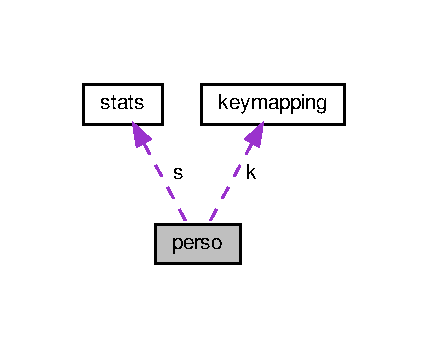
\includegraphics[width=206pt]{structperso__coll__graph}
\end{center}
\end{figure}
\subsection*{Attributs publics}
\begin{DoxyCompactItemize}
\item 
\mbox{\Hypertarget{structperso_a12fc662a43d623979458104aa64051d7}\label{structperso_a12fc662a43d623979458104aa64051d7}} 
S\+D\+L\+\_\+\+Surface $\ast$ {\bfseries p} \mbox{[}6\mbox{]}\mbox{[}4\mbox{]}
\item 
\mbox{\Hypertarget{structperso_a1702962d93240085dc2dfab4c0d7754f}\label{structperso_a1702962d93240085dc2dfab4c0d7754f}} 
S\+D\+L\+\_\+\+Rect {\bfseries pos}
\item 
\mbox{\Hypertarget{structperso_a76b41475467835b866812bdbaafb6909}\label{structperso_a76b41475467835b866812bdbaafb6909}} 
int {\bfseries direction}
\item 
\mbox{\Hypertarget{structperso_a9a114ad315d65e3c2e17b407eb080b91}\label{structperso_a9a114ad315d65e3c2e17b407eb080b91}} 
int {\bfseries previous\+\_\+direction}
\item 
\mbox{\Hypertarget{structperso_a7f75eb44b8c8bb04d499547fe9f0873c}\label{structperso_a7f75eb44b8c8bb04d499547fe9f0873c}} 
int {\bfseries num}
\item 
\mbox{\Hypertarget{structperso_a7276d0267b905e084a91f2c156fb46eb}\label{structperso_a7276d0267b905e084a91f2c156fb46eb}} 
int {\bfseries hp} \mbox{[}2\mbox{]}
\item 
\mbox{\Hypertarget{structperso_a00a7c864ddb8aed3d8a01e29c4ae0d7b}\label{structperso_a00a7c864ddb8aed3d8a01e29c4ae0d7b}} 
int {\bfseries score} \mbox{[}2\mbox{]}
\item 
\mbox{\Hypertarget{structperso_a16124d4b769b42483530bdcddfabb93a}\label{structperso_a16124d4b769b42483530bdcddfabb93a}} 
S\+D\+L\+\_\+\+Surface $\ast$ {\bfseries images\+\_\+hp} \mbox{[}2\mbox{]}\mbox{[}11\mbox{]}
\item 
\mbox{\Hypertarget{structperso_afc6ab25d4a7c812315486a94566a9fdb}\label{structperso_afc6ab25d4a7c812315486a94566a9fdb}} 
int {\bfseries pos\+\_\+absolue}
\item 
\mbox{\Hypertarget{structperso_a136cb618fb6a48f3d386bf358a575b74}\label{structperso_a136cb618fb6a48f3d386bf358a575b74}} 
S\+D\+L\+\_\+\+Surface $\ast$ {\bfseries background} \mbox{[}4\mbox{]}
\item 
\mbox{\Hypertarget{structperso_a30e99273ad4d5f5a50c72f1626cc405b}\label{structperso_a30e99273ad4d5f5a50c72f1626cc405b}} 
S\+D\+L\+\_\+\+Rect {\bfseries bg}
\item 
\mbox{\Hypertarget{structperso_a2215338309a931400f0863fd5041d82b}\label{structperso_a2215338309a931400f0863fd5041d82b}} 
int {\bfseries next}
\item 
\mbox{\Hypertarget{structperso_a41362c60ce965d63463fb5fe4aefb519}\label{structperso_a41362c60ce965d63463fb5fe4aefb519}} 
int {\bfseries jump}
\item 
\mbox{\Hypertarget{structperso_a436a62035d458f03e914f2a15e92064a}\label{structperso_a436a62035d458f03e914f2a15e92064a}} 
int {\bfseries cheat}
\item 
\mbox{\Hypertarget{structperso_a2330bb4058a3c590424f7b66f0a1d8ca}\label{structperso_a2330bb4058a3c590424f7b66f0a1d8ca}} 
int {\bfseries speed}
\item 
\mbox{\Hypertarget{structperso_aa711c3c9792b3d1463060046d31c2cf9}\label{structperso_aa711c3c9792b3d1463060046d31c2cf9}} 
int {\bfseries fade}
\item 
\mbox{\Hypertarget{structperso_a27424a1bed94325802586e357d724d4c}\label{structperso_a27424a1bed94325802586e357d724d4c}} 
int {\bfseries done}
\item 
\mbox{\Hypertarget{structperso_a7b43c3bd1fc7cc065dfd72963b4b8f5a}\label{structperso_a7b43c3bd1fc7cc065dfd72963b4b8f5a}} 
int {\bfseries jetpack}
\item 
\mbox{\Hypertarget{structperso_a72867eb87b2f920b5dd87644d08038a7}\label{structperso_a72867eb87b2f920b5dd87644d08038a7}} 
T\+T\+F\+\_\+\+Font $\ast$ {\bfseries font} \mbox{[}2\mbox{]}
\item 
\mbox{\Hypertarget{structperso_a739cb92b3c4545805a4406b29e0e96ed}\label{structperso_a739cb92b3c4545805a4406b29e0e96ed}} 
\hyperlink{structkeymapping}{keymapping} {\bfseries k}
\item 
\mbox{\Hypertarget{structperso_a6a7f79828e1dbda1bac692606193ec7e}\label{structperso_a6a7f79828e1dbda1bac692606193ec7e}} 
\hyperlink{structstats}{stats} {\bfseries s}
\item 
\mbox{\Hypertarget{structperso_ac932cb7616724b3cc343975fe7ee191d}\label{structperso_ac932cb7616724b3cc343975fe7ee191d}} 
int {\bfseries number}
\end{DoxyCompactItemize}


La documentation de cette structure a été générée à partir du fichier suivant \+:\begin{DoxyCompactItemize}
\item 
personnage.\+h\end{DoxyCompactItemize}

\hypertarget{structsaving}{}\section{Référence de la structure saving}
\label{structsaving}\index{saving@{saving}}


Graphe de collaboration de saving\+:\nopagebreak
\begin{figure}[H]
\begin{center}
\leavevmode
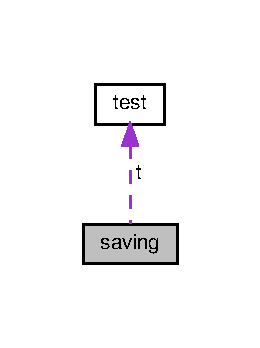
\includegraphics[width=125pt]{structsaving__coll__graph}
\end{center}
\end{figure}
\subsection*{Attributs publics}
\begin{DoxyCompactItemize}
\item 
\mbox{\Hypertarget{structsaving_aca94e80d9a13f26fbd0cf7a2b0209842}\label{structsaving_aca94e80d9a13f26fbd0cf7a2b0209842}} 
S\+D\+L\+\_\+\+Rect {\bfseries pos\+\_\+perso}
\item 
\mbox{\Hypertarget{structsaving_afcc79338d07307a3532e7466455608f5}\label{structsaving_afcc79338d07307a3532e7466455608f5}} 
S\+D\+L\+\_\+\+Rect {\bfseries pos\+\_\+bg}
\item 
\mbox{\Hypertarget{structsaving_af5f6643245e497f8764585c38b36ff86}\label{structsaving_af5f6643245e497f8764585c38b36ff86}} 
\hyperlink{structtest}{test} {\bfseries t} \mbox{[}3\mbox{]}
\item 
\mbox{\Hypertarget{structsaving_ac753d825770022e56ffbd1c2c520b844}\label{structsaving_ac753d825770022e56ffbd1c2c520b844}} 
int {\bfseries hp}
\end{DoxyCompactItemize}


La documentation de cette structure a été générée à partir du fichier suivant \+:\begin{DoxyCompactItemize}
\item 
personnage.\+h\end{DoxyCompactItemize}

\hypertarget{structsettings}{}\section{Référence de la structure settings}
\label{structsettings}\index{settings@{settings}}
\subsection*{Attributs publics}
\begin{DoxyCompactItemize}
\item 
\mbox{\Hypertarget{structsettings_a3b2a3f5514b31900eb51f1cfcdb35ccc}\label{structsettings_a3b2a3f5514b31900eb51f1cfcdb35ccc}} 
Uint32 {\bfseries screen}
\item 
\mbox{\Hypertarget{structsettings_ae7255a055460ef549908f1217e332102}\label{structsettings_ae7255a055460ef549908f1217e332102}} 
int {\bfseries sfx\+\_\+volume}
\item 
\mbox{\Hypertarget{structsettings_a4c38da107e921e1b38e95fd05b44cf8c}\label{structsettings_a4c38da107e921e1b38e95fd05b44cf8c}} 
int {\bfseries music\+\_\+volume}
\end{DoxyCompactItemize}


La documentation de cette structure a été générée à partir du fichier suivant \+:\begin{DoxyCompactItemize}
\item 
menu.\+h\end{DoxyCompactItemize}

\hypertarget{structstats}{}\section{Référence de la structure stats}
\label{structstats}\index{stats@{stats}}
\subsection*{Attributs publics}
\begin{DoxyCompactItemize}
\item 
\mbox{\Hypertarget{structstats_adaf1bb24116d3127367d6ca5320cbba8}\label{structstats_adaf1bb24116d3127367d6ca5320cbba8}} 
int {\bfseries e\+\_\+d}
\item 
\mbox{\Hypertarget{structstats_aabe3a10b9174d0b342fed555fc824966}\label{structstats_aabe3a10b9174d0b342fed555fc824966}} 
int {\bfseries r\+\_\+s}
\item 
\mbox{\Hypertarget{structstats_ad3fa3740a9f065a3888fb5d6a703c494}\label{structstats_ad3fa3740a9f065a3888fb5d6a703c494}} 
int {\bfseries l\+\_\+r}
\end{DoxyCompactItemize}


La documentation de cette structure a été générée à partir du fichier suivant \+:\begin{DoxyCompactItemize}
\item 
personnage.\+h\end{DoxyCompactItemize}

\hypertarget{structtest}{}\section{Référence de la structure test}
\label{structtest}\index{test@{test}}
\subsection*{Attributs publics}
\begin{DoxyCompactItemize}
\item 
\mbox{\Hypertarget{structtest_aa611d9a096a2e88565958b93ee42f480}\label{structtest_aa611d9a096a2e88565958b93ee42f480}} 
S\+D\+L\+\_\+\+Surface $\ast$ {\bfseries image}
\item 
\mbox{\Hypertarget{structtest_a02bc6760103ffe3f2f19e3cc85bd2f9a}\label{structtest_a02bc6760103ffe3f2f19e3cc85bd2f9a}} 
S\+D\+L\+\_\+\+Rect {\bfseries pos}
\item 
\mbox{\Hypertarget{structtest_ae2211e607f9dd448c1d6b35675a5bc8e}\label{structtest_ae2211e607f9dd448c1d6b35675a5bc8e}} 
int {\bfseries xmin}
\item 
\mbox{\Hypertarget{structtest_a7e81fb134868a8435fefdb916e63edd8}\label{structtest_a7e81fb134868a8435fefdb916e63edd8}} 
int {\bfseries xmax}
\item 
\mbox{\Hypertarget{structtest_a19776f2cddb45a7488d22b0fad7d372d}\label{structtest_a19776f2cddb45a7488d22b0fad7d372d}} 
int {\bfseries d}
\item 
\mbox{\Hypertarget{structtest_a371776b8b06dd040cb3b5fbe612b42f0}\label{structtest_a371776b8b06dd040cb3b5fbe612b42f0}} 
int {\bfseries num}
\item 
\mbox{\Hypertarget{structtest_a79b6aa09681f0d1b1b51e2ec1e6a6f7c}\label{structtest_a79b6aa09681f0d1b1b51e2ec1e6a6f7c}} 
int {\bfseries speed}
\item 
\mbox{\Hypertarget{structtest_a9160c293a819908aa0cd956bb0221bcc}\label{structtest_a9160c293a819908aa0cd956bb0221bcc}} 
int {\bfseries triggered}
\end{DoxyCompactItemize}


La documentation de cette structure a été générée à partir du fichier suivant \+:\begin{DoxyCompactItemize}
\item 
personnage.\+h\end{DoxyCompactItemize}

%--- End generated contents ---

% Index
\backmatter
\newpage
\phantomsection
\clearemptydoublepage
\addcontentsline{toc}{chapter}{Index}
\printindex

\end{document}
